\documentclass{article}
\usepackage{graphicx}
\usepackage{listings}
\usepackage{amsmath}
\usepackage{booktabs}
\usepackage{tabularx}
\usepackage{microtype}
\usepackage[hyphens]{url}
\usepackage[margin=1in]{geometry}

\sloppy
\emergencystretch=2em

\title{CS-455: The Right Word at the Right Time}
\author{
  Nuh Al-Sharafi\\
  \texttt{nuh.sharafi@sabanciuniv.edu}\\
  Student ID: 32702
  \and
  Musab Ahmed Khan\\
  \texttt{musab.khan@sabanciuniv.edu}\\
  Student ID: 33017
}
\date{June 2026}

\begin{document}

\maketitle

\begin{abstract}
We built \textit{The Right Word at the Right Time}, a terminal-based Turkish vocabulary recommender for learners who already know part of the language. The system indexes 50{,}000 high-frequency words from OpenSubtitles, retrieves candidates with a multilingual bi-encoder and FAISS, and reranks them with a lightweight multi-objective scorer. A separate chat mode adds an LLM tutor for explanations and follow-up questions. Benchmarks in \texttt{alpha.ipynb} over simulated learner profiles show that the weighted feature reranker consistently outperforms bi-encoder-only retrieval and a Turkish cross-encoder baseline on our evaluation metric. The best configuration (\texttt{paraphrase-multilingual-mpnet-base-v2}, mean embedding, weighted feature reranker) reached an average combined score of 0.671. The same pipeline is exposed through four CLI entry points, including a Rich-based study interface.
\end{abstract}

\section{Introduction}

The acquisition of a new language often presents a significant challenge for learners who have informally picked up foundational skills but lack a structured vocabulary. Traditional language learning platforms, such as Duolingo or standard textbooks, typically assume a ``zero-knowledge'' starting point, leading to a monotonous and repetitive experience for intermediate or informal learners. Conversely, skipping ahead often results in missing critical foundational gaps that were not covered during informal acquisition. This dichotomy highlights a pressing need for adaptive learning systems that can intelligently identify a user's current knowledge and recommend the exact ``next word'' required to advance.

This project introduces ``The Right Word at the Right Time,'' an adaptive neural retrieval system designed specifically for Turkish language learners. While traditional methods rely on static curriculum paths, this system leverages modern advancements in Large Language Models (LLMs) and semantic embeddings to create a dynamic recommendation pipeline. By modeling the Turkish language through a RAG-like architecture, the system provides personalized vocabulary suggestions based on semantic proximity to words the user already knows, filtered by frequency data derived from the OpenSubtitles Turkish dataset.

The primary objective is to build a terminal-based application that takes a list of a user's known words and outputs the most relevant next words to learn. Beyond simple recommendation, the system incorporates a decoder-based LLM to provide contextual definitions, translations, and example sentences, allowing for interactive clarifying questions. Because labeled ``next word'' data were not available, we evaluate ranking quality with intrinsic metrics on simulated learner profiles, comparing bi-encoder-only retrieval, weighted feature reranking, and a cross-encoder baseline. This approach aims to bridge the gap between informal language acquisition and organized proficiency through a scalable, neural-driven framework.

\section{Literature review}

Modeling an adaptive language acquisition system as a recommendation framework allows for the integration of recent computational advancements to design highly effective educational tools. The central challenge in this approach lies in understanding the individual learner's cognitive state to optimize the pedagogical utility of the recommendations. To address this, foundational inspiration is drawn from Lev Vygotsky's Zone of Proximal Development\cite{vygotsky1978mind} and Stephen Krashen's Input Hypothesis\cite{krashen1977monitor}, which together provide the theoretical basis for matching learners with appropriately challenging material. In addition to these theories, the work of Zhou and Wang\cite{zhou2025simulation} offers a compelling practical example of how dynamic learner states can be operationalized within a recommendation system for a different target language.

Lev Vygotsky's Zone of Proximal Development (ZPD)\cite{vygotsky1978mind} provides the psychological underpinning for adaptive instructional design. Vygotsky defined the ZPD as the cognitive distance between what a learner can achieve independently and what they can accomplish under the guidance of a ``More Knowledgeable Other'' or capable peers. Modern intelligent tutoring environments continuously calibrate the difficulty of vocabulary and tasks to keep the learner actively engaged in this optimal instructional ``sweet spot''. By dynamically providing personalized learning paths and adjusting content difficulty in real-time, AI-powered systems operationalize the ZPD to maximize cognitive growth and prevent both cognitive stagnation and overwhelming frustration.

Complementing the collaborative scaffolding of the ZPD, Stephen Krashen's Input Hypothesis\cite{krashen1977monitor} provides concrete guidance for the linguistic complexity of the recommended vocabulary. Krashen posited that second language acquisition is most effective when learners are exposed to ``comprehensible input'' that is slightly beyond their current level of linguistic competence, formalized as the i+1 level. If a learner's current competence is $i$, the optimal target for new input is $i+1$, allowing the learner to utilize context and existing knowledge to infer the meaning of unfamiliar elements without raising their ``affective filter'' (negative emotions that form a psychological barrier).

Providing a practical computational application of these pedagogical theories, Zhou and Wang\cite{zhou2025simulation} developed an online personalized English learning path recommendation system that integrates domain knowledge graphs with deep reinforcement learning. Their system captures both prerequisite and semantic relationships among knowledge points, utilizing graph-based propagation and an exponential forgetting mechanism to continuously update the learner's mastery state based on real-time interaction feedback. By formulating the recommendation task as a Markov Decision Process and employing a combination of Q-learning for value-based pruning and Proximal Policy Optimization (PPO) for action selection, their model effectively balances dynamic learner states with structured knowledge modeling. This framework demonstrates a successful architectural blueprint for how an adaptive system can continuously optimize personalized learning trajectories in a live educational environment. Unfortunately, their system is mostly beyond our scope for this project as we will only focus on vocabulary acquisition not whole language acquisition.

\section{Methodology}

\subsection{Data}
To develop a system tailored for Turkish language learners, we sought a dataset representative of everyday spoken Turkish. Consequently, we utilized the OpenSubtitles corpus \cite{lison-tiedemann-2016-opensubtitles2016}. Although this dataset is known to exhibit some translation artifacts, it provides an extensive and valuable resource comprising approximately 64 million sentences of conversational Turkish.

The preprocessing pipeline was adapted from a prior personal project in which the dataset was modeled as a bigram graph and structured into a relational database. This database consisted of two tables: a node table representing unique words and an edge table representing adjacent word pairs, with frequencies serving as weights. For the current project, only the node table (comprising lowercased words and their corresponding corpus frequencies) was utilized, and no lemmatization was performed. The initial parsing and database construction required approximately seven hours.

Once that database was ported, we used a bi-encoder \texttt{paraphrase-\allowbreak{}multilingual-\allowbreak{}mpnet-\allowbreak{}base-v2} to encode the words in the word-frequency table with \texttt{min\_weight} of 10 and \texttt{max\_vocab\_size} of 50{,}000. The embeddings were then stored in a FAISS inner-product index along with a word list for mapping the embeddings to the words. Additionally, a \texttt{meta.json} is generated with the configuration used to generate the embeddings; the CLI reads this file on startup so the same index is reused when parameters match.

\begin{lstlisting}[
    language=json,
    caption={Sample meta.json},
    label={lst:model_config}
]
{
  "bi_model": "sentence-transformers/paraphrase-multilingual-mpnet-base-v2",
  "min_weight": 10,
  "max_vocab_size": 50000,
  "num_vectors": 50000,
  "dimension": 768
}
\end{lstlisting}

\subsection{Design}

The system follows a two-phase pipeline, illustrated in Figure~\ref{fig:architecture}. An offline phase is run once to build a searchable semantic index from the corpus vocabulary, and an online phase runs at each session to produce personalized word recommendations for the learner.

In the offline phase, the word-frequency database is first loaded as described in the data section above.

At runtime, the learner's known words are maintained in a \textit{LearnerProfile} persisted as a JSON file. Before each query, a subset of the learner's known words is selected and aggregated into a single query vector. The default selection strategy, \textit{diverse}, draws from the middle and lower frequency bands of the learner's known vocabulary rather than the most common words, so that recommendations evolve as the learner acquires more vocabulary. An alternative \textit{topic} strategy selects known words whose embeddings are closest to a user-supplied topic keyword. Once a query vector is formed, the FAISS index is searched for the $k = 200$ nearest neighbors among unknown words, producing an initial candidate pool.

The candidate pool is then reranked by the \textit{WeightedFeatureReranker}. Drawing on the pedagogical framing in Section~2, we treat semantic proximity to known words as a proxy for comprehensible input \cite{krashen1977monitor}, frequency and difficulty terms as a proxy for staying near the learner's zone of proximal development rather than jumping too far ahead \cite{vygotsky1978mind}, and morphological overlap as related vocabulary in the same learning neighborhood. These objectives are combined in a weighted score (default weights $w_s{=}w_f{=}0.35$, $w_m{=}0.10$, $w_d{=}0.15$, $w_e{=}0.05$):
\begin{equation}
\label{eq:combined}
\text{score}(w) = w_s S + w_f F + w_m M - w_d D - w_e E
\end{equation}
where $S$ is bi-encoder semantic similarity, $F$ is normalized log-frequency utility, $M$ is morphological root overlap with known words (longest common prefix), $D$ is a diversity term, and $E$ is a difficulty penalty when the word is much rarer than the learner's average. The final suggestions are chosen iteratively via Maximum Marginal Relevance (MMR) \cite{carbonell1998mmr}: at each step the candidate with the highest $\text{score}(w)$ is picked, where $D$ is the maximum cosine similarity between $w$ and words already selected---so $D$ is \emph{subtracted} here to spread out the list.

An alternative cross-encoder reranker scores each candidate against a concatenated string of known words using \texttt{dbmdz/bert-base-turkish-cased}; benchmark results show it underperforms the weighted feature reranker on our evaluation metric.

When the LLM tutor is enabled, selected words are passed to an OpenRouter-hosted language model (by default \texttt{openrouter/free}), which provides a bilingual explanation and example sentences. Follow-up questions continue in a stateful conversation, and the word is added to the learner's profile upon confirmation.

\begin{figure}[t]
    \centering
    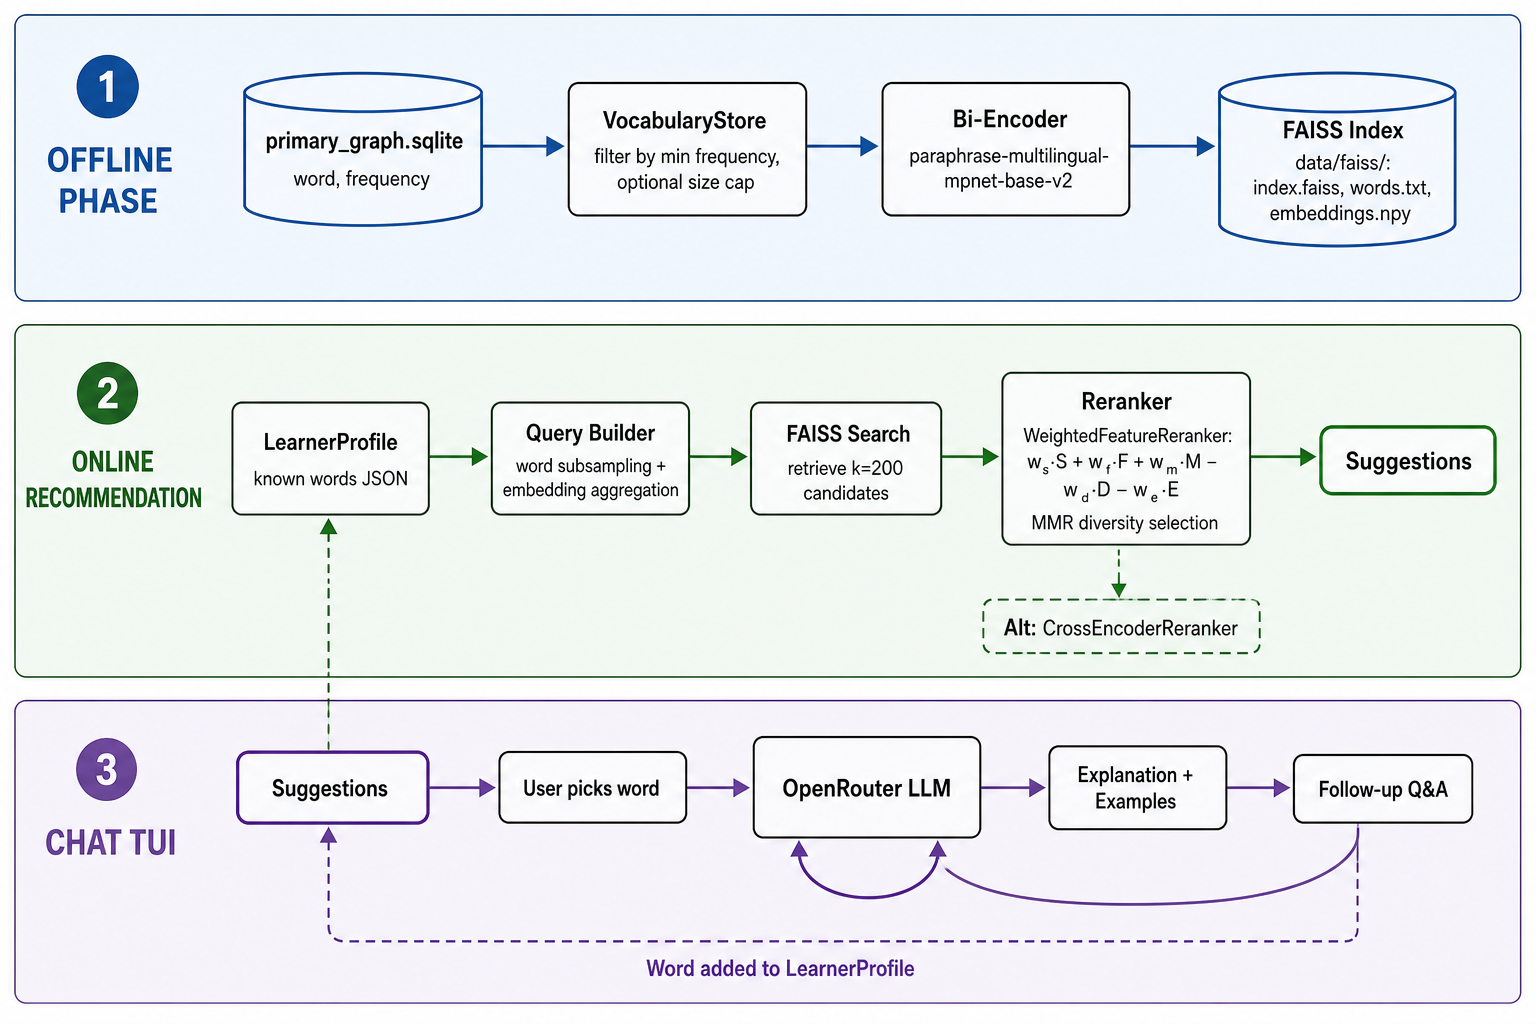
\includegraphics[width=\linewidth]{architecture.png}
    \caption{System architecture: offline index build and online retrieval, reranking, and optional LLM tutor.}
    \label{fig:architecture}
\end{figure}

\subsection{Interface}

In addition to being importable as a Python module, the system exposes four command-line entry points corresponding to different levels of engagement. \texttt{rwrt-build-index} is a one-time setup command that encodes the vocabulary and writes the FAISS artifacts to disk. \texttt{rwrt-recommend} is a stateless command that accepts a list of known words and prints the top suggestions, optionally loading and updating a learner profile. \texttt{rwrt-learn} wraps the same pipeline in an interactive loop where the learner can mark words as known one by one without making any LLM calls, suitable for offline or low-latency sessions. All three commands share a common set of flags for controlling the vocabulary filter, the number of candidates and final suggestions, the query strategy, and the reranker weights.

The primary interface is \texttt{rwrt-chat}, a terminal user interface built with the Rich library. Upon launch, the TUI displays a ranked table of suggestions showing each word alongside its bi-encoder score, weighted-feature score (\texttt{wf}), optional cross-encoder score, and corpus frequency. The learner interacts through a single input line: entering a number such as \texttt{4} opens that word for study, while appending \texttt{k} to a number (e.g.\ \texttt{1k, 2k}) marks it as already known without invoking the LLM. These actions can be combined, so a learner may type \texttt{1k, 2k, 3k, 4} to mark three words as known and immediately study the fourth. Pressing \texttt{r} refreshes the suggestion list, and \texttt{q} exits the session.

\begin{figure}[t]
    \centering
    \begin{minipage}{0.48\linewidth}
        \centering
        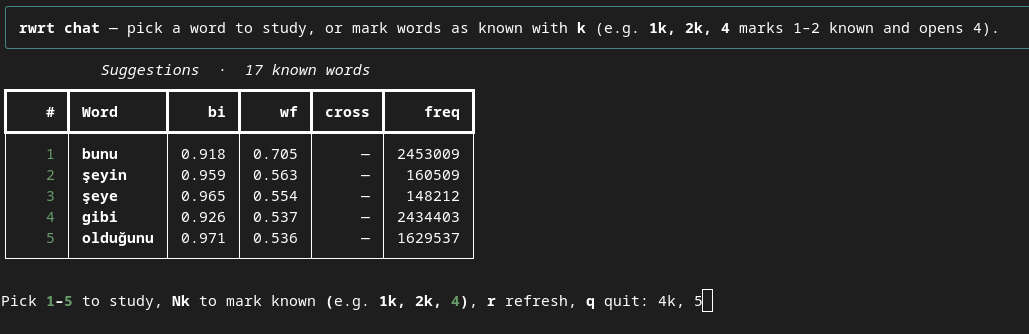
\includegraphics[width=\linewidth]{screenshot-1.png}
        \caption{Suggestion table in \texttt{rwrt-chat}.}
        \label{fig:screenshot-1}
    \end{minipage}\hfill
    \begin{minipage}{0.48\linewidth}
        \centering
        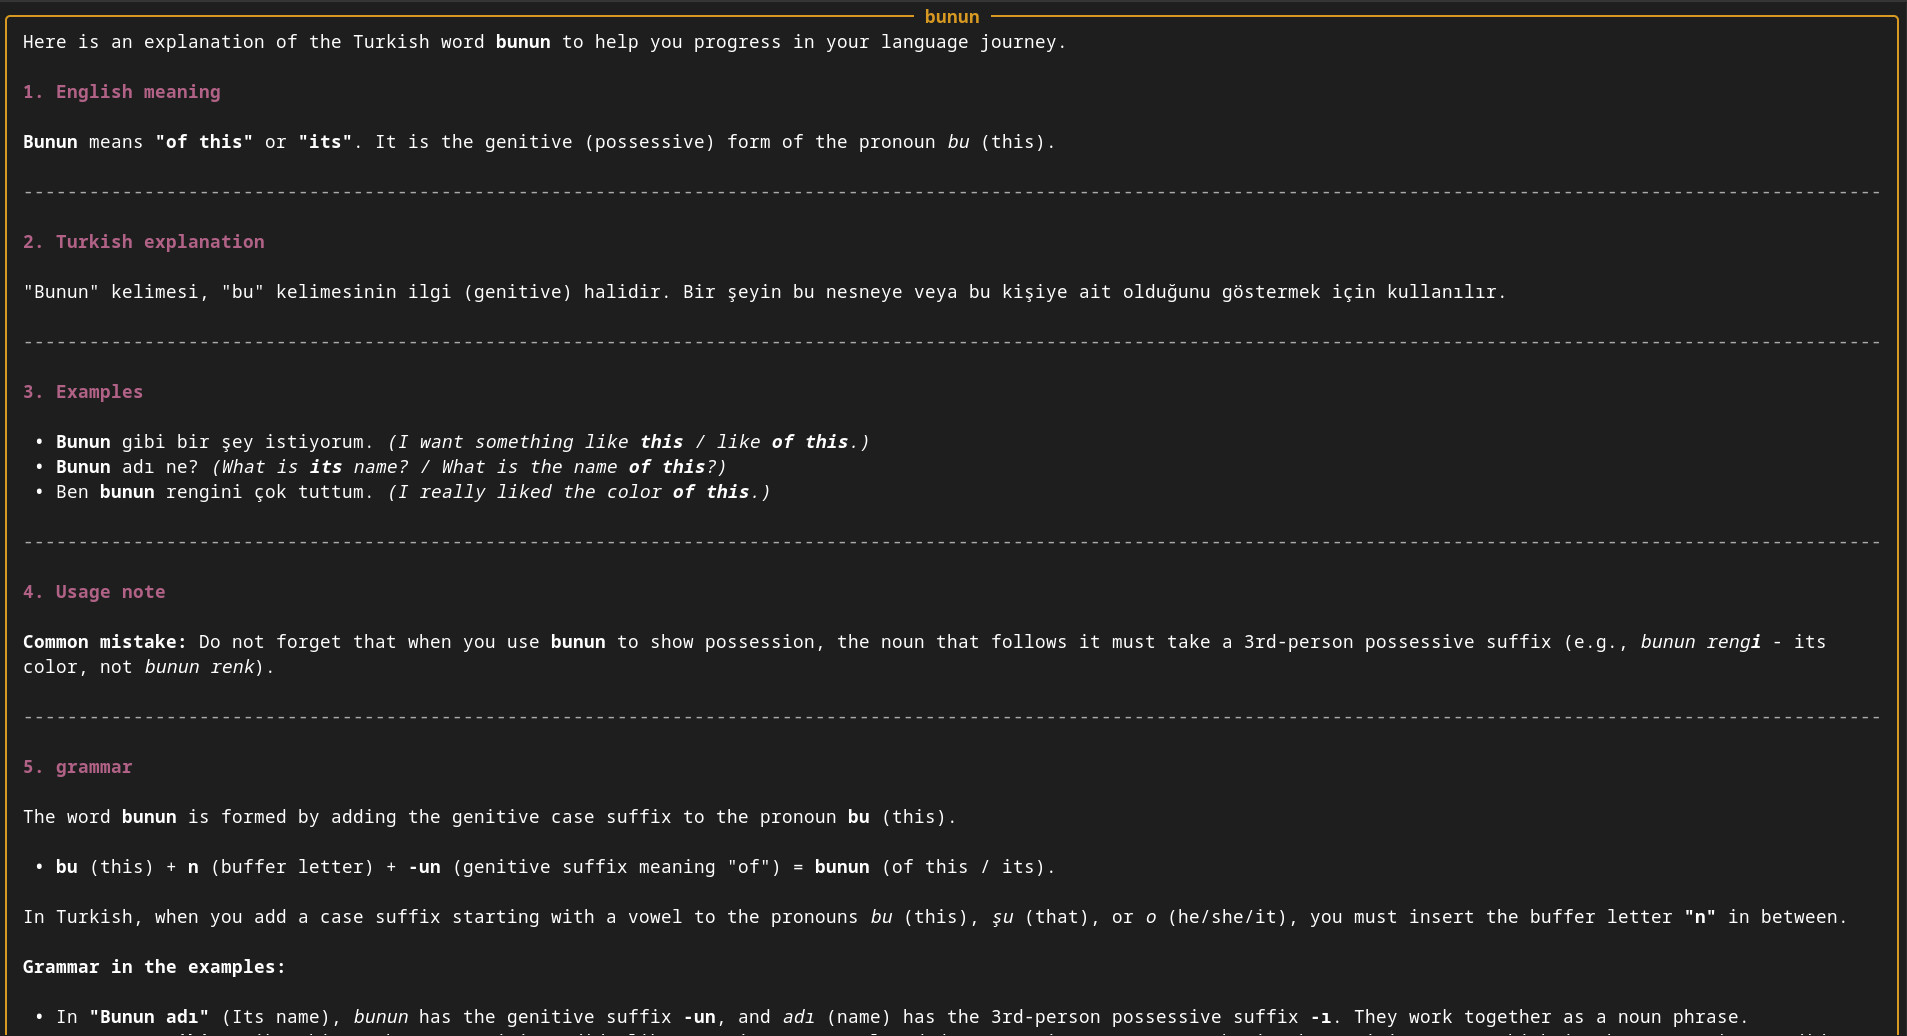
\includegraphics[width=\linewidth]{screenshot-3.png}
        \caption{LLM tutor explanation for a selected word.}
        \label{fig:screenshot-2}
    \end{minipage}
\end{figure}

When a word is opened for study, the LLM tutor produces an explanation in both English and Turkish with example sentences, rendered as formatted Markdown in the terminal (Figure~\ref{fig:screenshot-2}). The learner can then type follow-up questions in natural language. Pressing Enter on an empty line confirms that the word has been learned, adds it to the profile, and returns to the suggestion screen. Pressing \texttt{b} returns without recording the word as learned.

\section{Evaluation and Results}
\label{sec:eval}

\subsection{Evaluation setup}

Our original proposal planned ranking metrics such as Mean Reciprocal Rank (MRR) and Recall@10 against held-out ``next words.'' In practice we did not have reliable ground-truth labels for Turkish vocabulary progression at the word level, so we adopted an \textit{intrinsic} evaluation in \texttt{alpha.ipynb} instead.

We simulate learners by sampling known-word sets of sizes 10, 25, 50, 100, 200, and 500 (five random profiles per size), retrieve the top 10 unknown suggestions per profile, and score the resulting lists with the \textbf{same} combined formula (Equation~\eqref{eq:combined}), using the same default weights. The benchmark in \texttt{alpha.ipynb} averages each term over the ten recommended words rather than computing them per candidate at pick time. In practice the terms match the design intent: $S$ is semantic fit to known words, $F$ is frequency utility, $M$ is morphological relatedness, and $E$ penalizes overly rare words. The only subtlety is $D$: during reranking it is subtracted as an MMR penalty (maximum similarity to words already chosen), while in evaluation it is the diversity of the final list, defined as $1 - \text{mean pairwise cosine}$, and enters with a plus sign---so a \emph{diverse} cluster scores higher on $D$ in the benchmark. That is intentional for measuring variety; the reranker still uses subtraction to avoid duplicate neighbors at selection time. Each configuration is averaged over 30 profile runs; results are saved to \path{data/faiss_alpha/benchmark_results.json}.

We compared three bi-encoders (\texttt{paraphrase-multilingual-mpnet-base-v2}, \texttt{distiluse-base-multilingual-cased-v2}, \texttt{multilingual-e5-small}), three query strategies (\texttt{mean\_embedding}, \texttt{weighted\_mean}, \texttt{inverse\_weighted\_mean}), and three reranking modes: bi-encoder only, weighted feature reranker, and cross-encoder reranker. Cross-encoder runs were limited to the two larger models because of GPU memory and latency.

\subsection{Notebook benchmark results}

Table~\ref{tab:benchmark} summarizes representative configurations on mean combined score. The weighted feature reranker improves every bi-encoder and query-strategy pair we tested relative to bi-encoder-only retrieval. The cross-encoder reranker scores lower on the combined metric despite sometimes high $S$, because it does not optimize $F$, $M$, or $D$ directly.

\begin{table}[t]
\centering
\small
\begin{tabularx}{\linewidth}{>{\raggedright\arraybackslash}p{0.28\linewidth}p{0.22\linewidth}p{0.22\linewidth}r}
\toprule
Bi-encoder & Query strategy & Reranker & Avg.\ combined \\
\midrule
mpnet & mean\_embedding & weighted feature & \textbf{0.671} \\
mpnet & mean\_embedding & bi-encoder only  & 0.598 \\
mpnet & mean\_embedding & cross-encoder    & 0.580 \\
mpnet & inv.\ weighted mean & weighted feature & 0.666 \\
e5-small & mean\_embedding & weighted feature & 0.653 \\
distiluse & mean\_embedding & weighted feature & 0.643 \\
\bottomrule
\end{tabularx}
\caption{Representative benchmark averages (30 profiles per row). Full grid in \texttt{alpha.ipynb}.}
\label{tab:benchmark}
\end{table}

On the best configuration, weighted feature reranking raised the average combined score from 0.598 to 0.671 (+12.3\%). Sub-metric averages for that run were $S{=}0.955$, $F{=}0.691$, $M{=}0.880$, $D{=}0.049$, and $E{=}0.000$. Larger simulated profiles tended to score higher (Figure~\ref{fig:profilesize}). The smaller e5 model reached 0.653 with weighted feature reranking, suggesting a lighter deployment option at modest quality cost.

Figure~\ref{fig:benchmark-reranker} plots mean combined score for each bi-encoder and reranking mode (mean-embedding query strategy). Weighted feature reranking is highest for every model; the cross-encoder trails despite strong semantic scores on some runs. Figure~\ref{fig:submetrics} decomposes the winning mpnet configuration: high $S$ and $M$ with a small positive contribution from list diversity $D$. Figure~\ref{fig:heatmap-wf} shows that weighted feature scores are relatively stable across query strategies for mpnet and e5-small, with a slight edge for mean embedding on the best model. Figure~\ref{fig:freq-scatter} relates combined score to frequency appropriateness across all runs. Figure~\ref{fig:radar-methods} compares sub-metrics for bi-only, weighted feature, and cross-encoder on the best model and query strategy.

\begin{figure}[t]
    \centering
    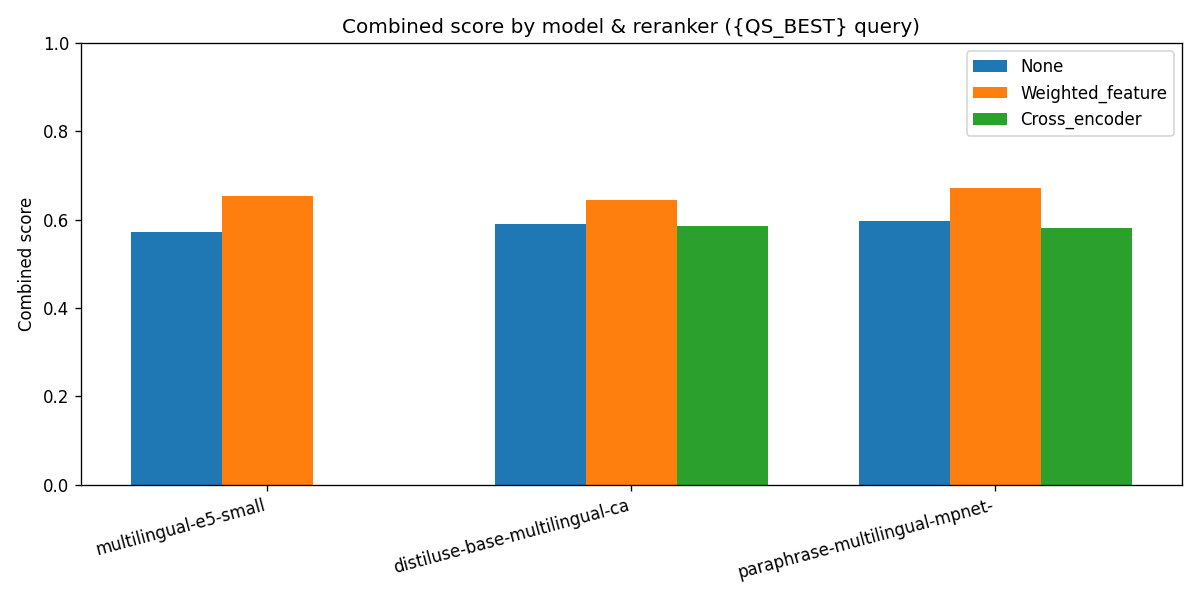
\includegraphics[width=\linewidth]{fig_combined_by_model_reranker.png}
    \caption{Mean combined evaluation score by bi-encoder and reranker (\texttt{mean\_embedding} query), from \texttt{alpha.ipynb}.}
    \label{fig:benchmark-reranker}
\end{figure}

\begin{figure}[t]
    \centering
    \begin{minipage}{0.48\linewidth}
        \centering
        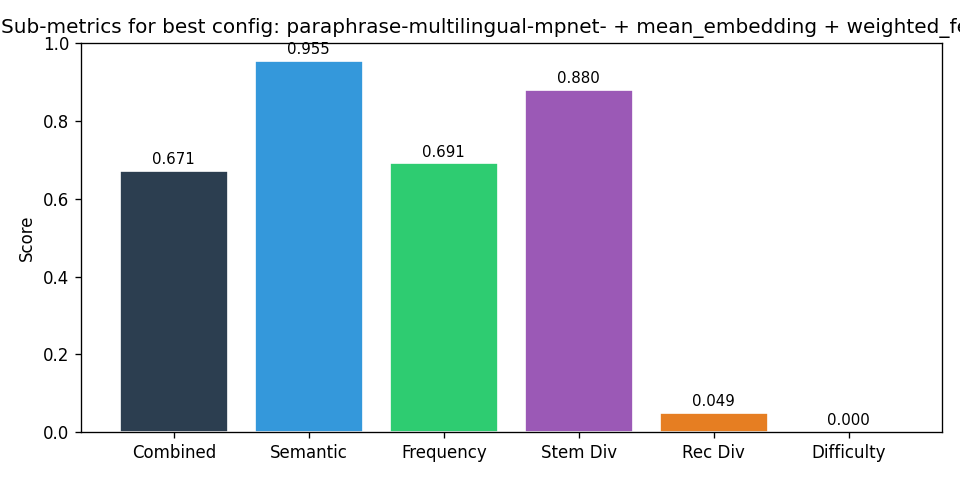
\includegraphics[width=\linewidth]{fig_submetrics_best_config.png}
        \caption{Sub-metric breakdown for the best configuration (mpnet, mean embedding, weighted feature).}
        \label{fig:submetrics}
    \end{minipage}\hfill
    \begin{minipage}{0.48\linewidth}
        \centering
        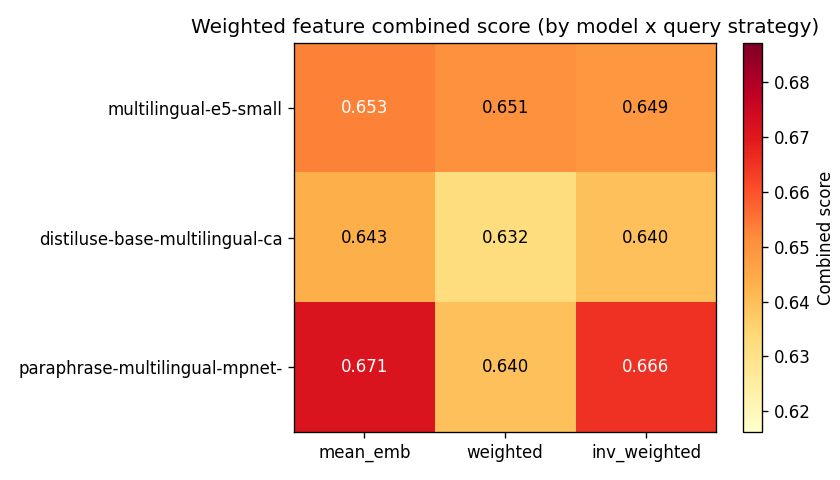
\includegraphics[width=\linewidth]{fig_heatmap_model_strategy.png}
        \caption{Weighted-feature combined score across models and query strategies.}
        \label{fig:heatmap-wf}
    \end{minipage}
\end{figure}

\begin{figure}[t]
    \centering
    \begin{minipage}{0.48\linewidth}
        \centering
        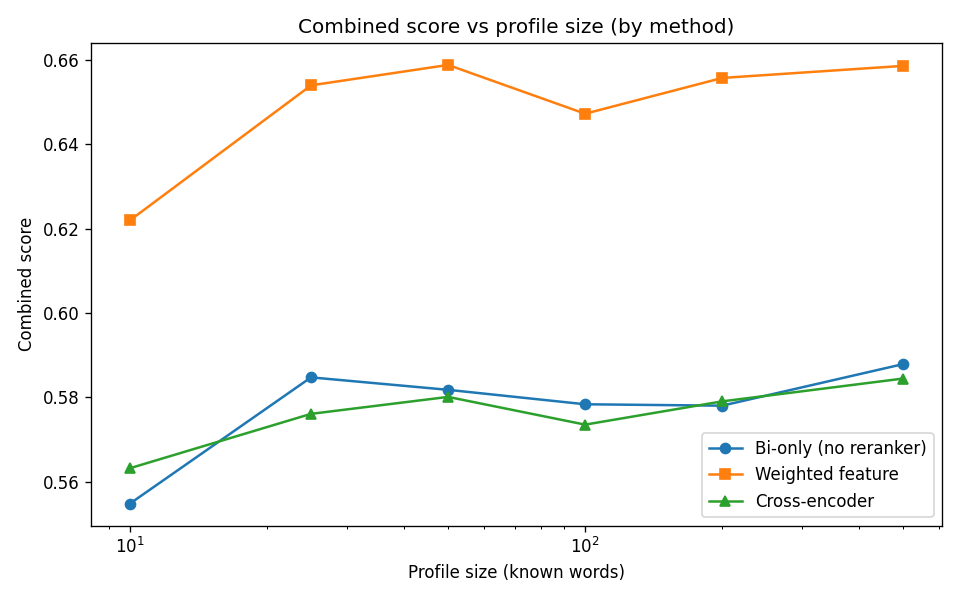
\includegraphics[width=\linewidth]{fig_combined_vs_profilesize.png}
        \caption{Combined score vs.\ simulated profile size (by reranking method).}
        \label{fig:profilesize}
    \end{minipage}\hfill
    \begin{minipage}{0.48\linewidth}
        \centering
        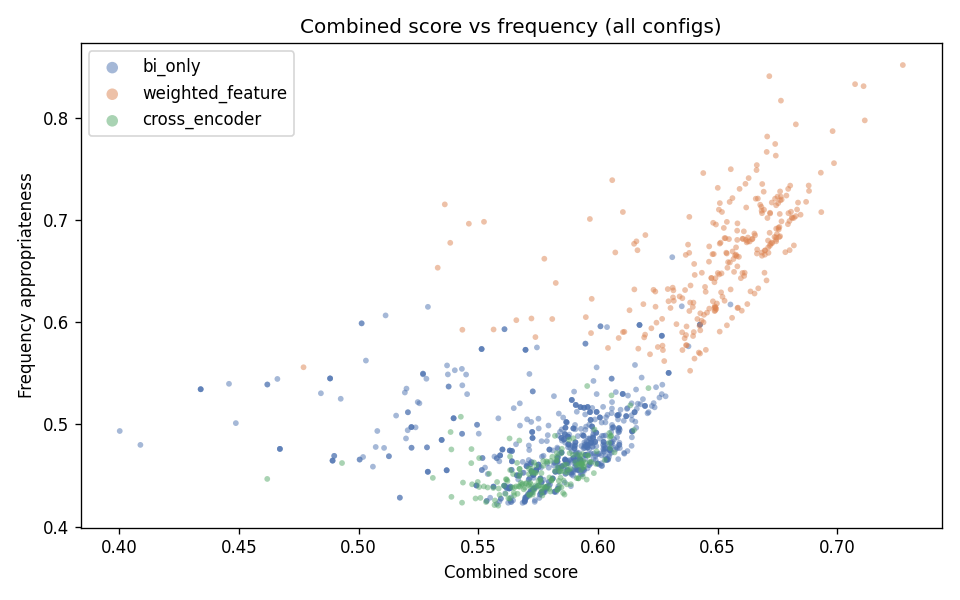
\includegraphics[width=\linewidth]{fig_combined_vs_freq_scatter.png}
        \caption{Combined score vs.\ frequency appropriateness (all configurations).}
        \label{fig:freq-scatter}
    \end{minipage}
\end{figure}

\begin{figure}[t]
    \centering
    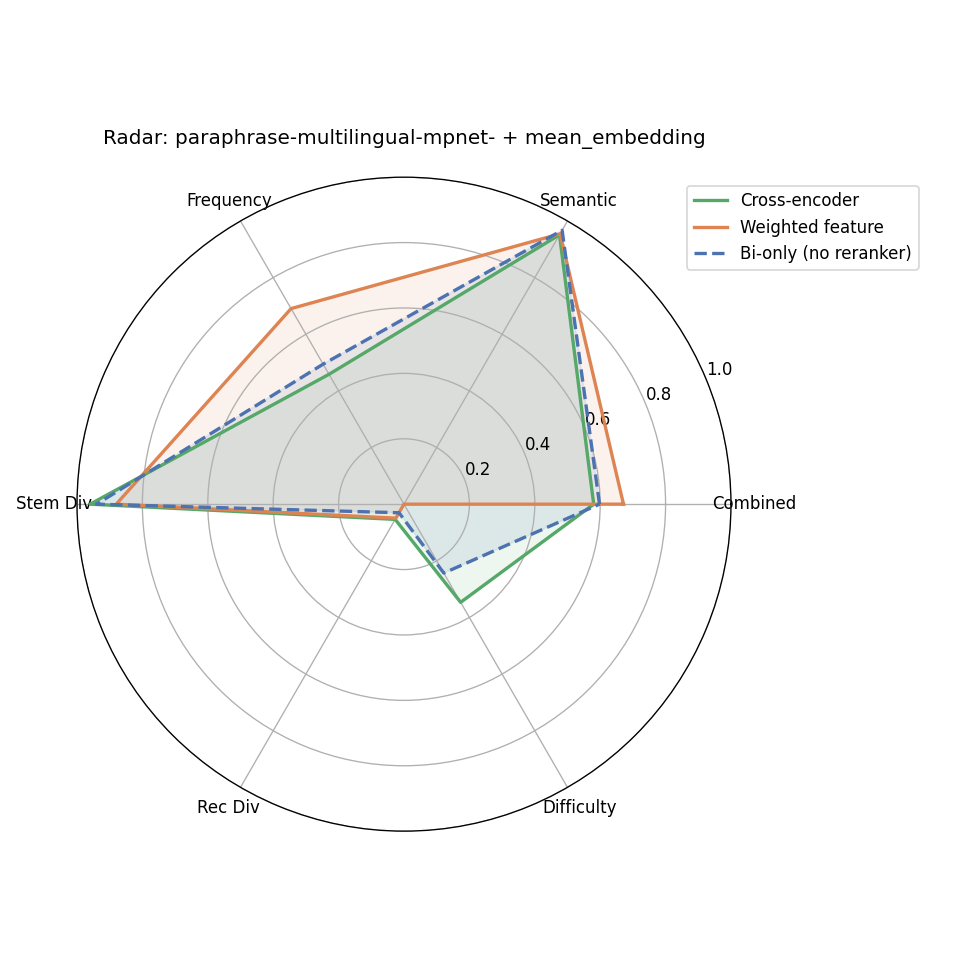
\includegraphics[width=0.62\linewidth]{fig_radar_cross_vs_weighted.png}
    \caption{Radar of mean sub-metrics on the best model and query strategy: bi-encoder only, weighted feature, and cross-encoder. Cross-encoder can lead on $S$ but loses on $F$, $M$, and $D$.}
    \label{fig:radar-methods}
\end{figure}

Qualitative checks in the notebook's topic section (keywords such as \textit{yemek}, \textit{seyahat}, \textit{okul}) showed that weighted feature suggestions often share stems with the topic word (e.g.\ \textit{okula}, \textit{okulda} for \textit{okul}), while cross-encoder picks were less morphologically aligned.

\subsection{CLI demonstration}

The \texttt{rwrt} package mirrors the notebook pipeline in four command-line tools, all sharing \texttt{PipelineConfig} defaults and override flags.

\textbf{One-shot recommend (\texttt{rwrt-recommend}).}
A quick demo: \texttt{rwrt-recommend merhaba teşekkür evet kitap -n 5} loads the cached mpnet index, applies weighted feature reranking, and prints ranked words with \texttt{bi=}, \texttt{wf=}, \texttt{cross=}, and \texttt{freq=} columns. The \texttt{wf} value is the reranking score from Equation~\eqref{eq:combined} (including MMR). \texttt{cross=} is empty unless \texttt{--reranker-type cross\_encoder} is set. With \texttt{--bi-only}, output follows pure FAISS order---useful for comparing against the default.

\textbf{Interactive learn (\texttt{rwrt-learn}).}
Same recommender in a text loop without LLM calls; the learner picks a numbered suggestion and the word is appended to a JSON profile.

\textbf{Chat tutor (\texttt{rwrt-chat}).}
The Rich TUI (Figure~\ref{fig:screenshot-1}) combines recommendations with an OpenRouter-backed tutor (\texttt{.env} API key). Selecting a word triggers a bilingual explanation; follow-up questions are supported before the word is saved to the profile.

\textbf{Index build (\texttt{rwrt-build-index}).}
Indexes live under \path{data/faiss/<model_slug>/} with \path{meta.json}. The CLI auto-resolves the correct subfolder when \path{data/faiss} is passed. A smoke script (\path{scripts/run_all_checks.sh}) and 88 pytest cases cover the Python API.

\section{Discussion}

Weighted feature reranking gave the strongest results on our evaluation metric. The cross-encoder checkpoint (\texttt{dbmdz/bert-base-turkish-cased}) is a masked-language model without a head trained for this ranking task; CLI runs with \texttt{--reranker-type cross\_encoder} often surface weak or unrelated neighbors. Semantic similarity alone is not enough: learners also need appropriate frequency, morphological relatedness, and variety in the suggestion list.

The shift from MRR/Recall to intrinsic metrics was necessary given our data, but it limits direct comparison to the original proposal. Future work could add human ratings or a small labeled set of acceptable next words per profile.

The terminal interfaces evolved through several iterations: early versions required manual index paths and did not show reranker scores in the output table. The final CLI prints separate \texttt{wf} and \texttt{cross} columns so it is clear which stage produced each value.

\subsection{What didn't work}

%talk about how the terminal interface kept having to be upgraded to allow overriding different parameters.
%talk about how many times I had to redesign the package to have defaults, overrideable by env, overrideable by terminal parameters for maximum flexibility.
One of the big design pain points was configurability where we spent 3 full days designing and re-designing the \texttt{rwrt} package until it got to a point where we were happy with it. We wanted to have a very flexible package with sensible defaults. The defaults had to be in one place. That place had to be clear, clean and small. We also wanted to have a \texttt{.env} file, that should override the defaults. We also wanted to be able to override both the \texttt{.env} and defaults using command line parameters. We wanted to be able to switch searching strategies and models on the fly, so everything had to be very standardized. The point of this was to make testing and benchmarking as easy as possible. AI helped a lot in seeing some of the ideas through which taught us where our mistakes were and allowed us to quickly iterate through solutions.

%talk about how the terminal interface kept having to be upgraded to allow overriding different parameters.
The terminal interface also went through several upgrades. Early demos could not override index paths, vocabulary caps, or reranker settings from the command line, which made side-by-side comparisons slow. Later versions added shared flags across \texttt{rwrt-recommend}, \texttt{rwrt-learn}, and \texttt{rwrt-chat}, plus automatic resolution of per-model FAISS subdirectories under \path{data/faiss/}.

%talk about how the metrics had to be reselected
Our original evaluation plan relied on MRR and Recall@10 against held-out next words, but we lacked a trustworthy labeled set at the word level. We moved to the intrinsic combined metric in Equation~\eqref{eq:combined}, with stem diversity and list-level diversity terms added after inspecting early suggestion lists that were semantically close but morphologically repetitive.

%talk about how the cross-encoder didn't work
The cross-encoder path did not work as well as we hoped. The Turkish BERT checkpoint is not trained as a relevance ranker for ``known words $\rightarrow$ next word,'' and load-time warnings indicate a randomly initialized classification head. It remained in the project as an optional baseline (\texttt{--reranker-type cross\_encoder}) rather than the default.

%talk about rec diversity metric tension
List-level \textit{rec diversity} ($D$) also caused confusion during benchmarking. We first had the sign wrong in \texttt{alpha.ipynb} ($D$ was reporting mean pairwise similarity instead of $1 - \text{mean sim}$), which made the best runs look artificially diverse until we fixed it. After the fix, $D$ on the winning configuration was still low ($\approx 0.05$), i.e.\ recommended words remain very close in embedding space (mean pairwise cosine $\approx 0.95$). That is not a reranker bug: retrieval and reranking are built to keep suggestions near the learner's known-word neighborhood, and high semantic coherence ($S \approx 0.95$) tends to imply low embedding spread among the top ten. MMR subtracts similarity only to words already chosen at pick time, which helps slightly on average ($D \approx 0.08$ with weighted feature vs.\ $\approx 0.05$ bi-only) but does not optimize the same quantity as the evaluation metric. Stem diversity can still be high while $D$ stays low, because Turkish inflections look different by prefix overlap but cluster in the same semantic region. We kept $w_d = 0.15$ as a light nudge rather than forcing unrelated words that would hurt $S$.

\subsection{AI use}

Cursor was used in the development of the \texttt{rwrt} module to speed up the process and adhere to high portability standards. All the code was thoroughly reviewed and tested to make sure it aligned with the vision and gave the expected outputs.

%Insert paragraph about musab's use of AI.
Opencode assistance was used to help with notebook experiment scaffolding, plotting, and drafting parts of the evaluation narrative in \texttt{alpha.ipynb}. Benchmark numbers and configuration tables were verified against saved JSON outputs.

Finally, openwebUI was used to help with rephrasing some parts of this report to ensure the tone remained professional. It goes without saying that the accuracy of the output was checked against reality before being transferred into this report.

\section{Conclusion}

We delivered a working Turkish vocabulary recommender with an offline FAISS index, a default multi-objective reranker, optional cross-encoder comparison, and three CLI usage modes (one-shot, interactive learn, LLM chat). The best automated configuration, mpnet, mean embedding, weighted feature reranking, achieved a combined evaluation score of 0.671 on simulated profiles, ahead of bi-encoder-only (0.598) and cross-encoder (0.580) baselines on the same metric. The system is suitable for terminal-based demos; sensible next steps are human evaluation, lemmatization-aware morphology, and a fine-tuned cross-encoder if pairwise reranking remains a goal.

\clearpage
\bibliographystyle{plain}
\bibliography{references}

\end{document}
